\documentclass[a4paper,11pt,titlepage]{jsarticle}
\usepackage[final]{graphicx}
\usepackage[dvipdfmx]{color}
\usepackage{listings, xcolor}
\usepackage{amsmath}
\usepackage{here}
\usepackage{tikz}

\lstset{
    basicstyle = {\ttfamily},
    frame = {tbrl},
    breaklines = true,
    numbers = left,
    showspaces = false,
    showstringspaces = false,
    showtabs = false,
    keywordstyle = \color{blue},
    commentstyle = {\color[HTML]{1AB91A}},
    identifierstyle = \color{black},
    stringstyle = \color{brown},
    captionpos = t
}

\title{画像処理レポート3}
\author{235738B 越後 玲輝}

\begin{document}

\maketitle
\newpage

\section{トーンカーブ変換}
\subsection{プログラム}
今回作成したプログラムは以下のとおり、
ルックアップテーブルを作成することで、処理の効率化を図った。
\lstinputlisting[caption=tone\_curve.py]{tone_curve.py}

\subsection{実行結果}
\begin{center}
  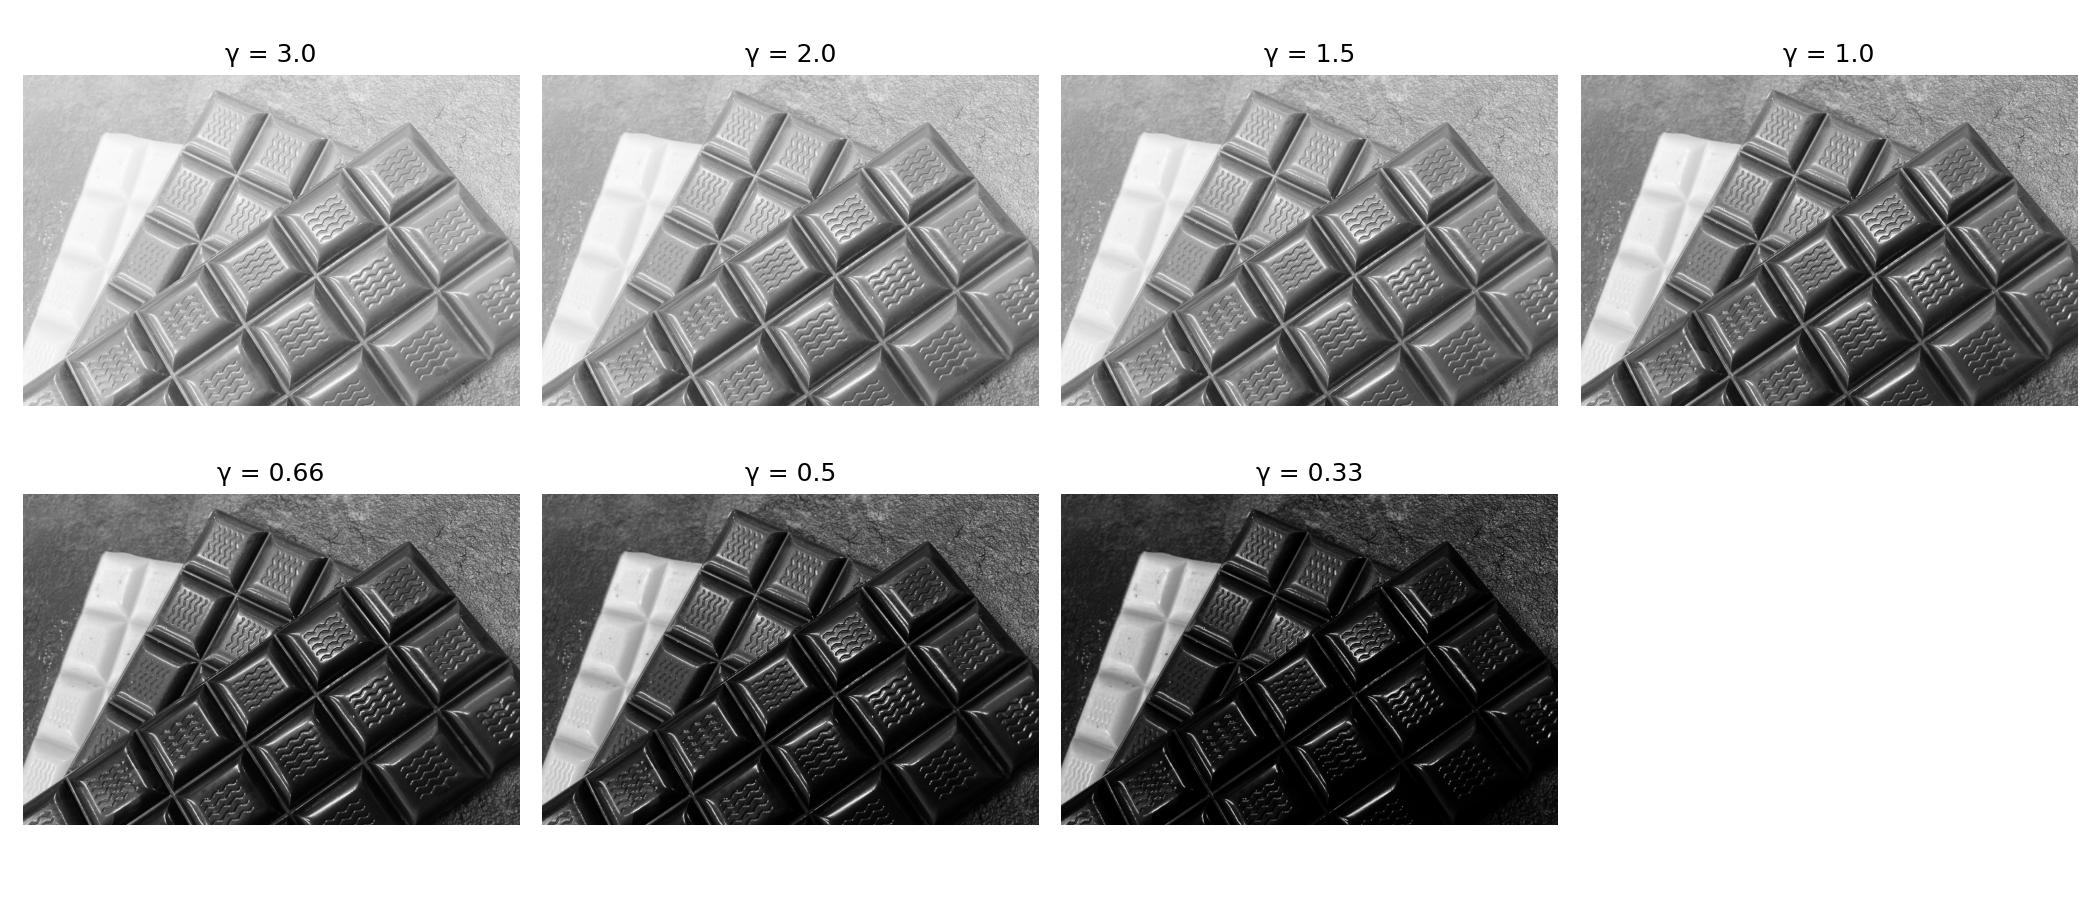
\includegraphics[width=0.8\linewidth]{gamma_gray_all.jpg} 
\end{center}

\section{カラー画像に対して適用。カラーチャンネル毎に適用。}
\subsection{カラー画像に対して、$\gamma$ = 0.5変換}
\begin{center}
  \includegraphics[width=0.8\linewidth]{gammma_color} 
\end{center}

\subsection{カラーチャンネルごとに変換(R = 1.8, G=0.7, B=0.4 )}
\begin{center}
  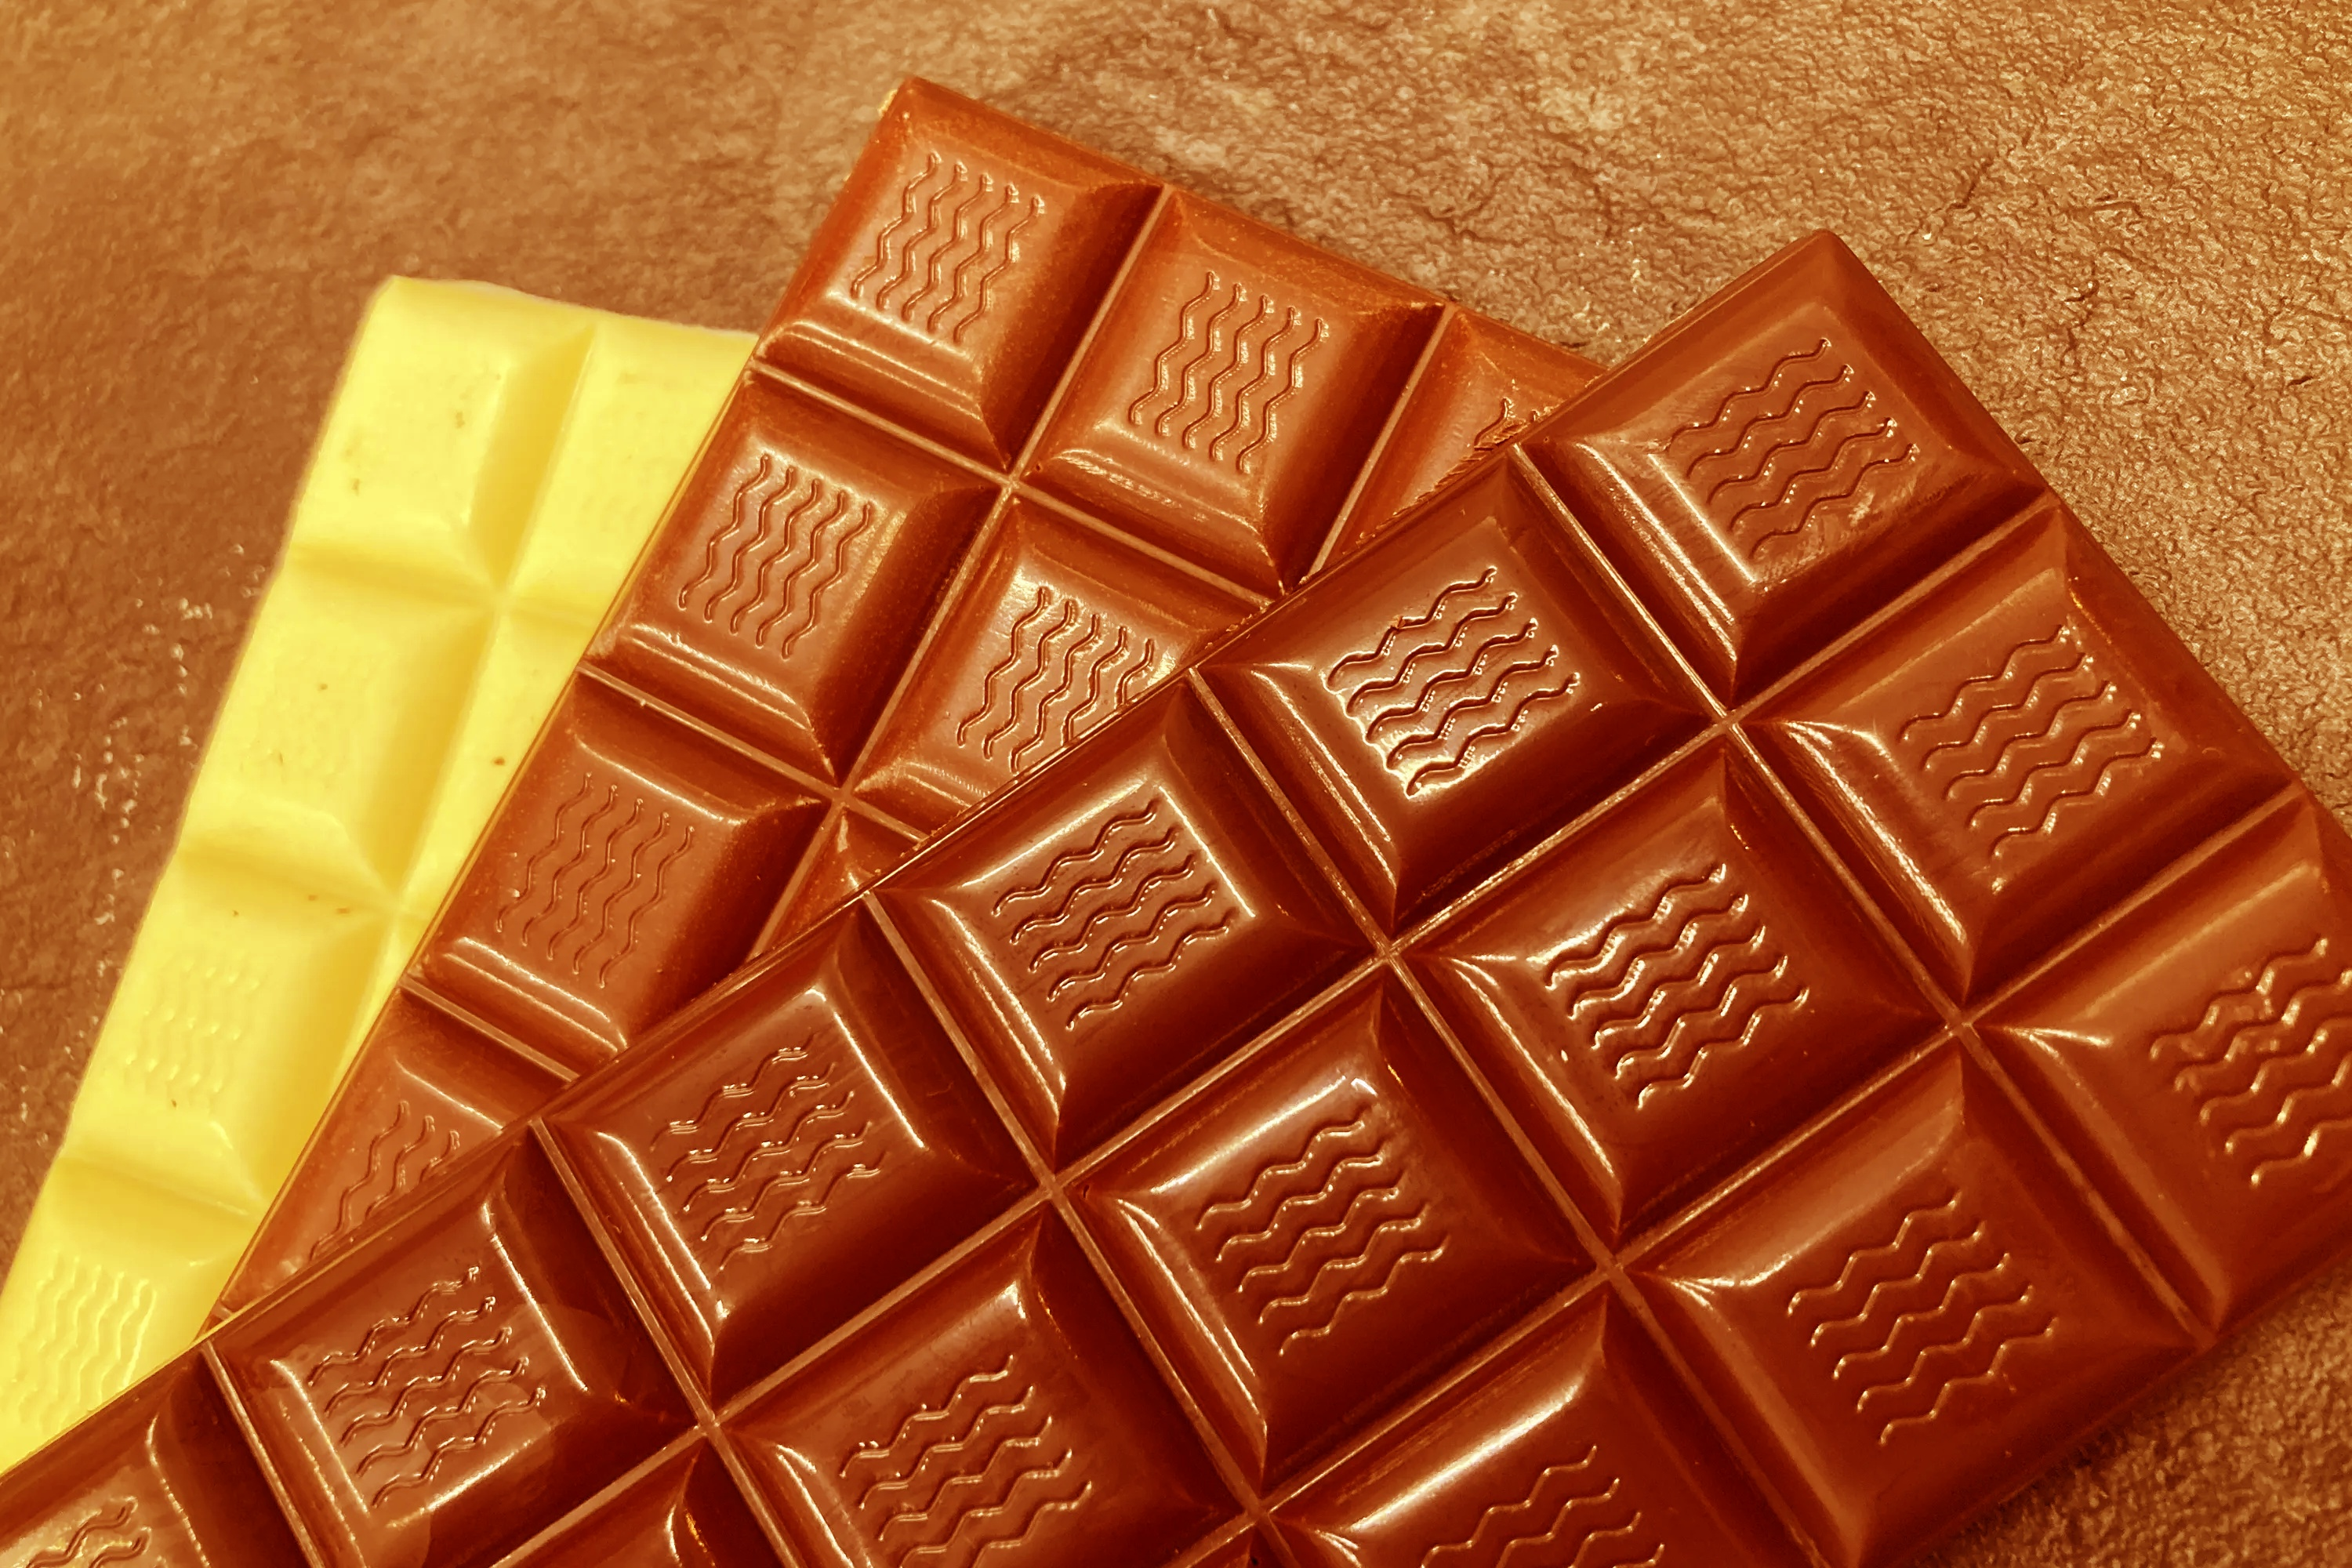
\includegraphics[width=0.8\linewidth]{gamma_color_fantasy.jpg} 
\end{center}

\section{αブレンディングを実行するプログラム作成}
\subsection{平均値ブレンド}
\lstinputlisting[caption=tone\_curve.py]{brend.py}

出力画像
\begin{center}
  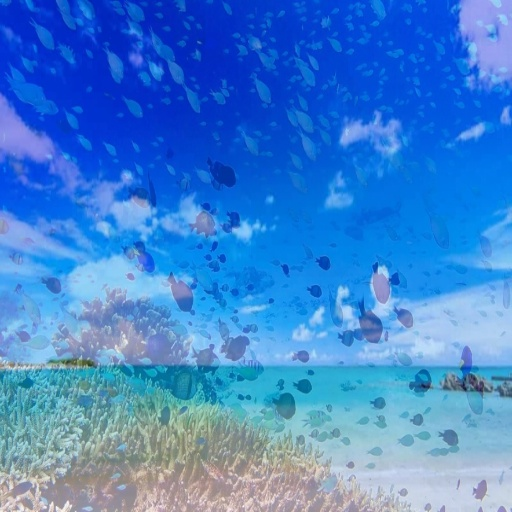
\includegraphics[width=0.8\linewidth]{alpha_fixed.jpg} 
\end{center}

\subsection{グラデブレンド(左から右)}
\lstinputlisting[caption=tone\_curve.py]{a_brend.py}

出力画像
\begin{center}
  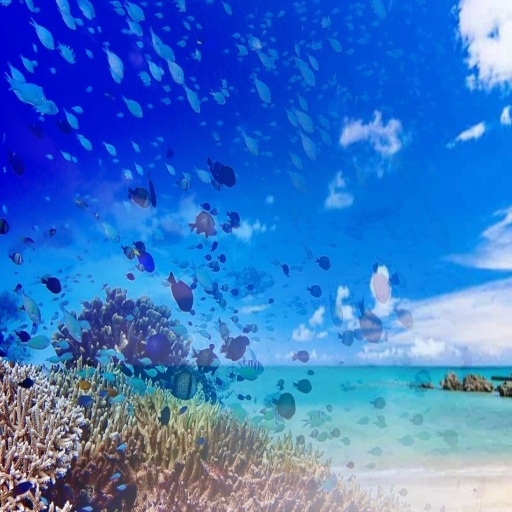
\includegraphics[width=0.8\linewidth]{alpha_gradient.jpg} 
\end{center}

\section{中心軸に関して左右反転}
プログラムは以下
\lstinputlisting[caption=tone\_curve.py]{/Users/reiki/workSpace/imageStu/report3/mirror.py}

出力画像
\begin{center}
  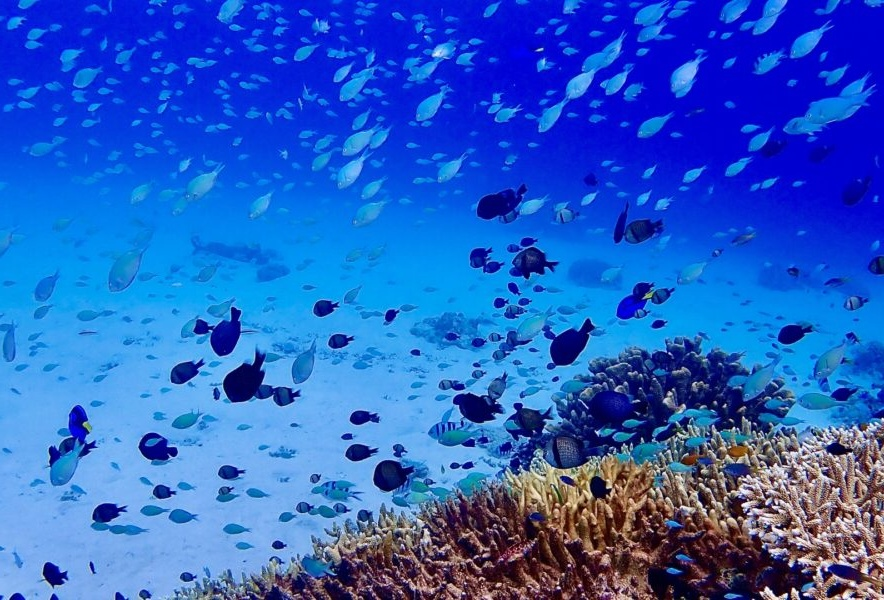
\includegraphics[width=0.8\linewidth]{flipped_image.jpg} 
\end{center}

\clearpage

\section{タイル状に区切って、各タイルを順番に左右反転表示}
プログラムは以下
\lstinputlisting[caption=tone\_curve.py]{tile_mirror.py}

\clearpage

出力画像
\begin{center}
  \includegraphics[width=0.8\linewidth]{mosaic_mirror} 
\end{center}

\end{document}
